\begin{pastexam}[label={px:ntu-109-comm-dsa-45}]{臺大電信所 109 學年度（B）第 45 題}
（複選；每題 2 分，每答錯一個選項倒扣 0.4 分）

Consider the splay tree in Fig.2.
\begin{enumerate}[label=(\Alph*),nosep]
\item In Fig.2, after inserting the key 93, then the parent of key 83 is key 79.
\item In Fig.2, after inserting the key 80, then the parent of key 80 is key 79.
\item In Fig.2, after inserting the key 33, then the parent of key 35 is key 48.
\item In Fig.2, after inserting the key 1, then the parent of key 15 is key 2.
\item In Fig.2, after inserting the key 40, then the root is key 40.
\end{enumerate}

\begin{center}
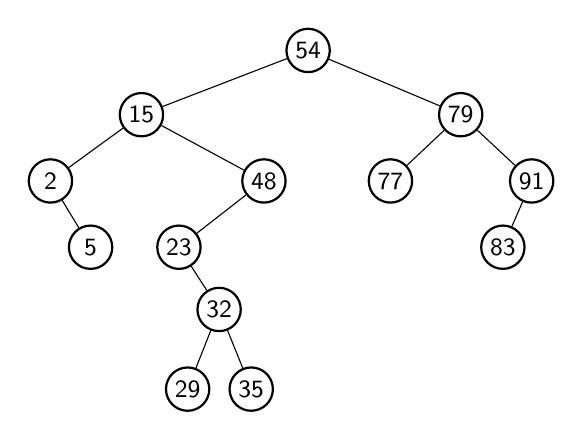
\begin{tikzpicture}[scale=0.85, v/.style={circle,draw,minimum size=5.5mm,inner sep=0pt,font=\small\sffamily,thick}]
\node[v] (54) at (5.92,-8.56) {54};
\node[v] (15) at (3.43,-9.52) {15};
\node[v] (79) at (8.20,-9.52) {79};
\node[v] (2) at (2.07,-10.51) {2};
\node[v] (48) at (5.26,-10.51) {48};
\node[v] (77) at (7.15,-10.51) {77};
\node[v] (91) at (9.26,-10.51) {91};
\node[v] (5) at (2.67,-11.50) {5};
\node[v] (23) at (3.99,-11.50) {23};
\node[v] (83) at (8.83,-11.50) {83};
\node[v] (32) at (4.59,-12.43) {32};
\node[v] (29) at (4.12,-13.62) {29};
\node[v] (35) at (5.07,-13.62) {35};
\draw (54) -- (15); \draw (54) -- (79);
\draw (15) -- (2); \draw (15) -- (48);
\draw (79) -- (77); \draw (79) -- (91);
\draw (2) -- (5); \draw (48) -- (23); \draw (91) -- (83);
\draw (23) -- (32); \draw (32) -- (29); \draw (32) -- (35);
\end{tikzpicture}

Fig.2 Splay tree
\end{center}
\end{pastexam}

\begin{pastsoln}
答案：(A)(C)(D)(E)。

依資結書第~10.6~節的做法：插入時先照二元搜尋樹插成葉節點，再把新節點由下而上（bottom-up）
伸展到根。 每一步看新節點 $x$、父節點 $p$、祖父節點 $g$：沒有 $g$ 做 zig；$x$、$p$ 同一側
做 zig-zig（先轉 $p$ 再轉 $x$）；不同側做 zig-zag（轉 $x$ 兩次）。 插入之後新的鍵一定是根。
下面用 $r(L, R)$ 表示根 $r$、左子樹 $L$、右子樹 $R$，「--」表示空。 原樹是
\[
54\bigl(15(2(\text{--}, 5),\ 48(23(\text{--}, 32(29, 35)), \text{--})),\ 79(77, 91(83, \text{--}))\bigr).
\]

\textbf{(A) 插入 93：對。} $93 > 54, 79, 91$，插成 $91$ 的右子節點。 $x = 93$、$p = 91$、
$g = 79$，都是右邊，zig-zig：先轉 $91$ 到 $79$ 的位置（$79$ 成為 $91$ 的左子節點，帶著 $77$、
$83$），再轉 $93$ 上去，得 $93(91(79(77, 83), \text{--}), \text{--})$ 掛在 $54$ 右邊。 接著
$p = 54$ 是根，zig，最後
\[
93\bigl(54(15(\ldots),\ 91(79(77, 83), \text{--})),\ \text{--}\bigr).
\]
$83$ 原本是 $91$ 的左子節點，第一次旋轉時 $91$ 往上、$83$ 改掛到 $79$ 的右邊，所以 $83$ 的父
節點是 $79$。

\textbf{(B) 插入 80：錯。} 插入後 $80$ 被伸展成根，根沒有父節點。 （就算不伸展，$80$ 插在
$83$ 的左邊，父節點也是 $83$ 不是 $79$。） 過程：$80$ 插成 $83$ 的左子節點；$80$、$83$、$91$
都在左邊，zig-zig 得 $80(\text{--}, 83(\text{--}, 91))$ 掛在 $79$ 右邊；再對 $80$、$79$、$54$
（都在右邊）做 zig-zig，結果 $80\bigl(79(54(15(\ldots), 77), \text{--}),\ 83(\text{--}, 91)\bigr)$。

\textbf{(C) 插入 33：對。} $33$ 走 $54 \to 15 \to 48 \to 23 \to 32 \to 35$，插成 $35$ 的左子節點。
三步都是 zig-zag：
\begin{enumerate}
\item $x = 33$、$p = 35$（$32$ 的右子節點）、$g = 32$：$33$ 上到 $32$ 的位置，左邊 $32(29, \text{--})$，
右邊 $35$，得 $33(32(29, \text{--}), 35)$，掛在 $23$ 的右邊。
\item $p = 23$（$48$ 的左子節點）、$g = 48$：$33$ 上去，左邊 $23(\text{--}, 32(29, \text{--}))$，右邊
$48(35, \text{--})$。 $33$ 原來的右子樹 $35$ 改掛成 $48$ 的左子節點。
\item $p = 15$（$54$ 的左子節點）、$g = 54$：$33$ 成為根，左邊 $15(2(\text{--}, 5), 23(\ldots))$，
右邊 $54(48(35, \text{--}), 79(\ldots))$。
\end{enumerate}
最後 $35$ 是 $48$ 的左子節點，父節點是 $48$。

\textbf{(D) 插入 1：對。} $1$ 插成 $2$ 的左子節點。 $x = 1$、$p = 2$、$g = 15$ 都在左邊，zig-zig：
先轉 $2$ 上去（$15$ 成為 $2$ 的右子節點，$2$ 原本的右子節點 $5$ 改掛成 $15$ 的左子節點），再轉
$1$ 上去，得 $1(\text{--}, 2(\text{--}, 15(5, 48(\ldots))))$。 最後對 $54$ 做 zig，$1$ 成為根，
$54$ 成為 $1$ 的右子節點，$2$ 改掛成 $54$ 的左子節點。 $15$ 的父節點是 $2$。

\textbf{(E) 插入 40：對。} 不管伸展的過程，bottom-up 伸展的定義就是把新插入的節點轉到根，所以
根是 $40$。 （過程：$40$ 插成 $35$ 的右子節點，對 $35$、$32$ 做 zig-zig，再做兩次 zig-zag，得
$40\bigl(15(2(\text{--}, 5), 23(\text{--}, 35(32(29, \text{--}), \text{--}))),\ 54(48, 79(\ldots))\bigr)$。）

\textbf{另一種做法。} 如果用由上而下（top-down）伸展來插入（例如 Weiss 的課本），(A)(B)(D)(E)
的判斷不變，但 (C) 插入 $33$ 後 $35$ 會成為 $33$ 的右子節點，(C) 變成錯的。 題目沒有指定，本書
照常見的 bottom-up 做法作答。
\end{pastsoln}
